%
% 公立はこだて未来大学卒業研究中間報告書[全コース対応版]
%
%         ファイル名:"sample.tex"
%
\documentclass[11pt]{ujarticle}
\usepackage{funinfosys}
\usepackage{url}
\usepackage[dvipdfmx]{graphicx}

\author{% 
1020259 中村碧\\指導教員 : 松原克弥
}
\course{Intelligent Systems Course}

\title{Wii Fit BoardとSphero SPRK+による直感的なロボット制御のためのMROS2の活用}
\etitle{}
\eauthor{Aoi Nakamura}
\abstract{ロボットソフトウェア開発において、ROS(Robot Operating System)の利用が増えている。ROSはクラウドサーバと連携し、分散型ロボットシステムを構築するのに役立つ。しかし、各機能モジュール(ノード)の配置はシステム稼働前に決定する必要があり、予測困難な状況変化で最適なノード配置が変わる可能性がある。クラウドとロボット間でのCPUアーキテクチャの違いにより、稼働中のノードの再配置は技術的に難しい。
\\この研究では、ROSノードの動的配置機構の実現に向けた、組み込みデバイス向けROS 2ランタイム実装であるmROS 2-Posixを評価する。mROS 2-PosixがROS 2と比較してマイグレーションに優位性があるかを明らかにし、動的配置機構の実現への影響を実験結果で示す。
}
\keywords{ロボティクス,mROS2}
\eabstract{
\\}
\ekeywords{Roboethics, mROS2}
\begin{document}
\maketitle
%\vspace*{-.5cm}

\section{背景と目的}
さまざまな産業向けやエンターテイメント関連のロボットシステム、自動車の自動運転技術やIoTシステムの構築においても、これらのソフトウェア開発をサポートするフレームワークとしてRobot Operating System(以下、ROS)の利用が増加している[1]。ROSのプログラミングモデルは、システムの各機能を独立したプログラムモジュール(ノード)として設計することにより、汎用性と再利用性を向上させて、各機能モジュール間のデータ交換を規定することで、効率的かつ柔軟なシステム構築を可能にしている。たとえば、カメラを操作して周囲の環境を撮影するノード、画像からオブジェクトを識別するノード、オブジェクトのデータを基に動作制御を実行するノードを連携させることで、自動運転車の基本機能の一部を容易に実装できる。
\\ ROSのプログラミングモデルは、ロボット/IoTとクラウドが協力する分散型システムにおいても有効である。ロボットシステムのソフトウェア処理は、「センサー」「知能・制御系」「動力系」の3要素に分けられる[2]。クラウドロボティクスにおいて[3]、主に知能・制御系のノードを高い計算能力を持つクラウドに優先して配置することで、高度な知能・制御処理の実現を促進し、さらに、必要な情報をクラウドに集約・保存することで、複数のロボット間での情報共有と利用を容易にする。
一方で、現行のROS実装においては、各ノードの配置をシステム起動時に設定する必要があり、先述のクラウドロボティクスのクラウドとロボット間の最適なノード配置を事前に設計する必要がある。しかし、実際の環境で動作するロボットは、ネットワークの状況やバッテリー残量の変動など、システム運用前に予測することが困難な状況変化に対応する必要があり、設定したクラウドとロボット間のノード配置が最適でなくなる可能性がある。このような状況変化に対する対応として、ノードを動的に再配置するマイグレーション機能の実現が求められているが、多くの場合でクラウドとロボット間のCPUアーキテクチャが異なり、実行中のノードをシステム運用中にマイグレーションすることは技術的に困難である。
\\ 本研究では,クラウドとロボット間での実行状態を含む稼働中ノードの動的マイグレーションの実現に向けたmROS 2-Posixの評価を行う.
%目的



\section{スクレイピング}


\begin{figure}[h]
	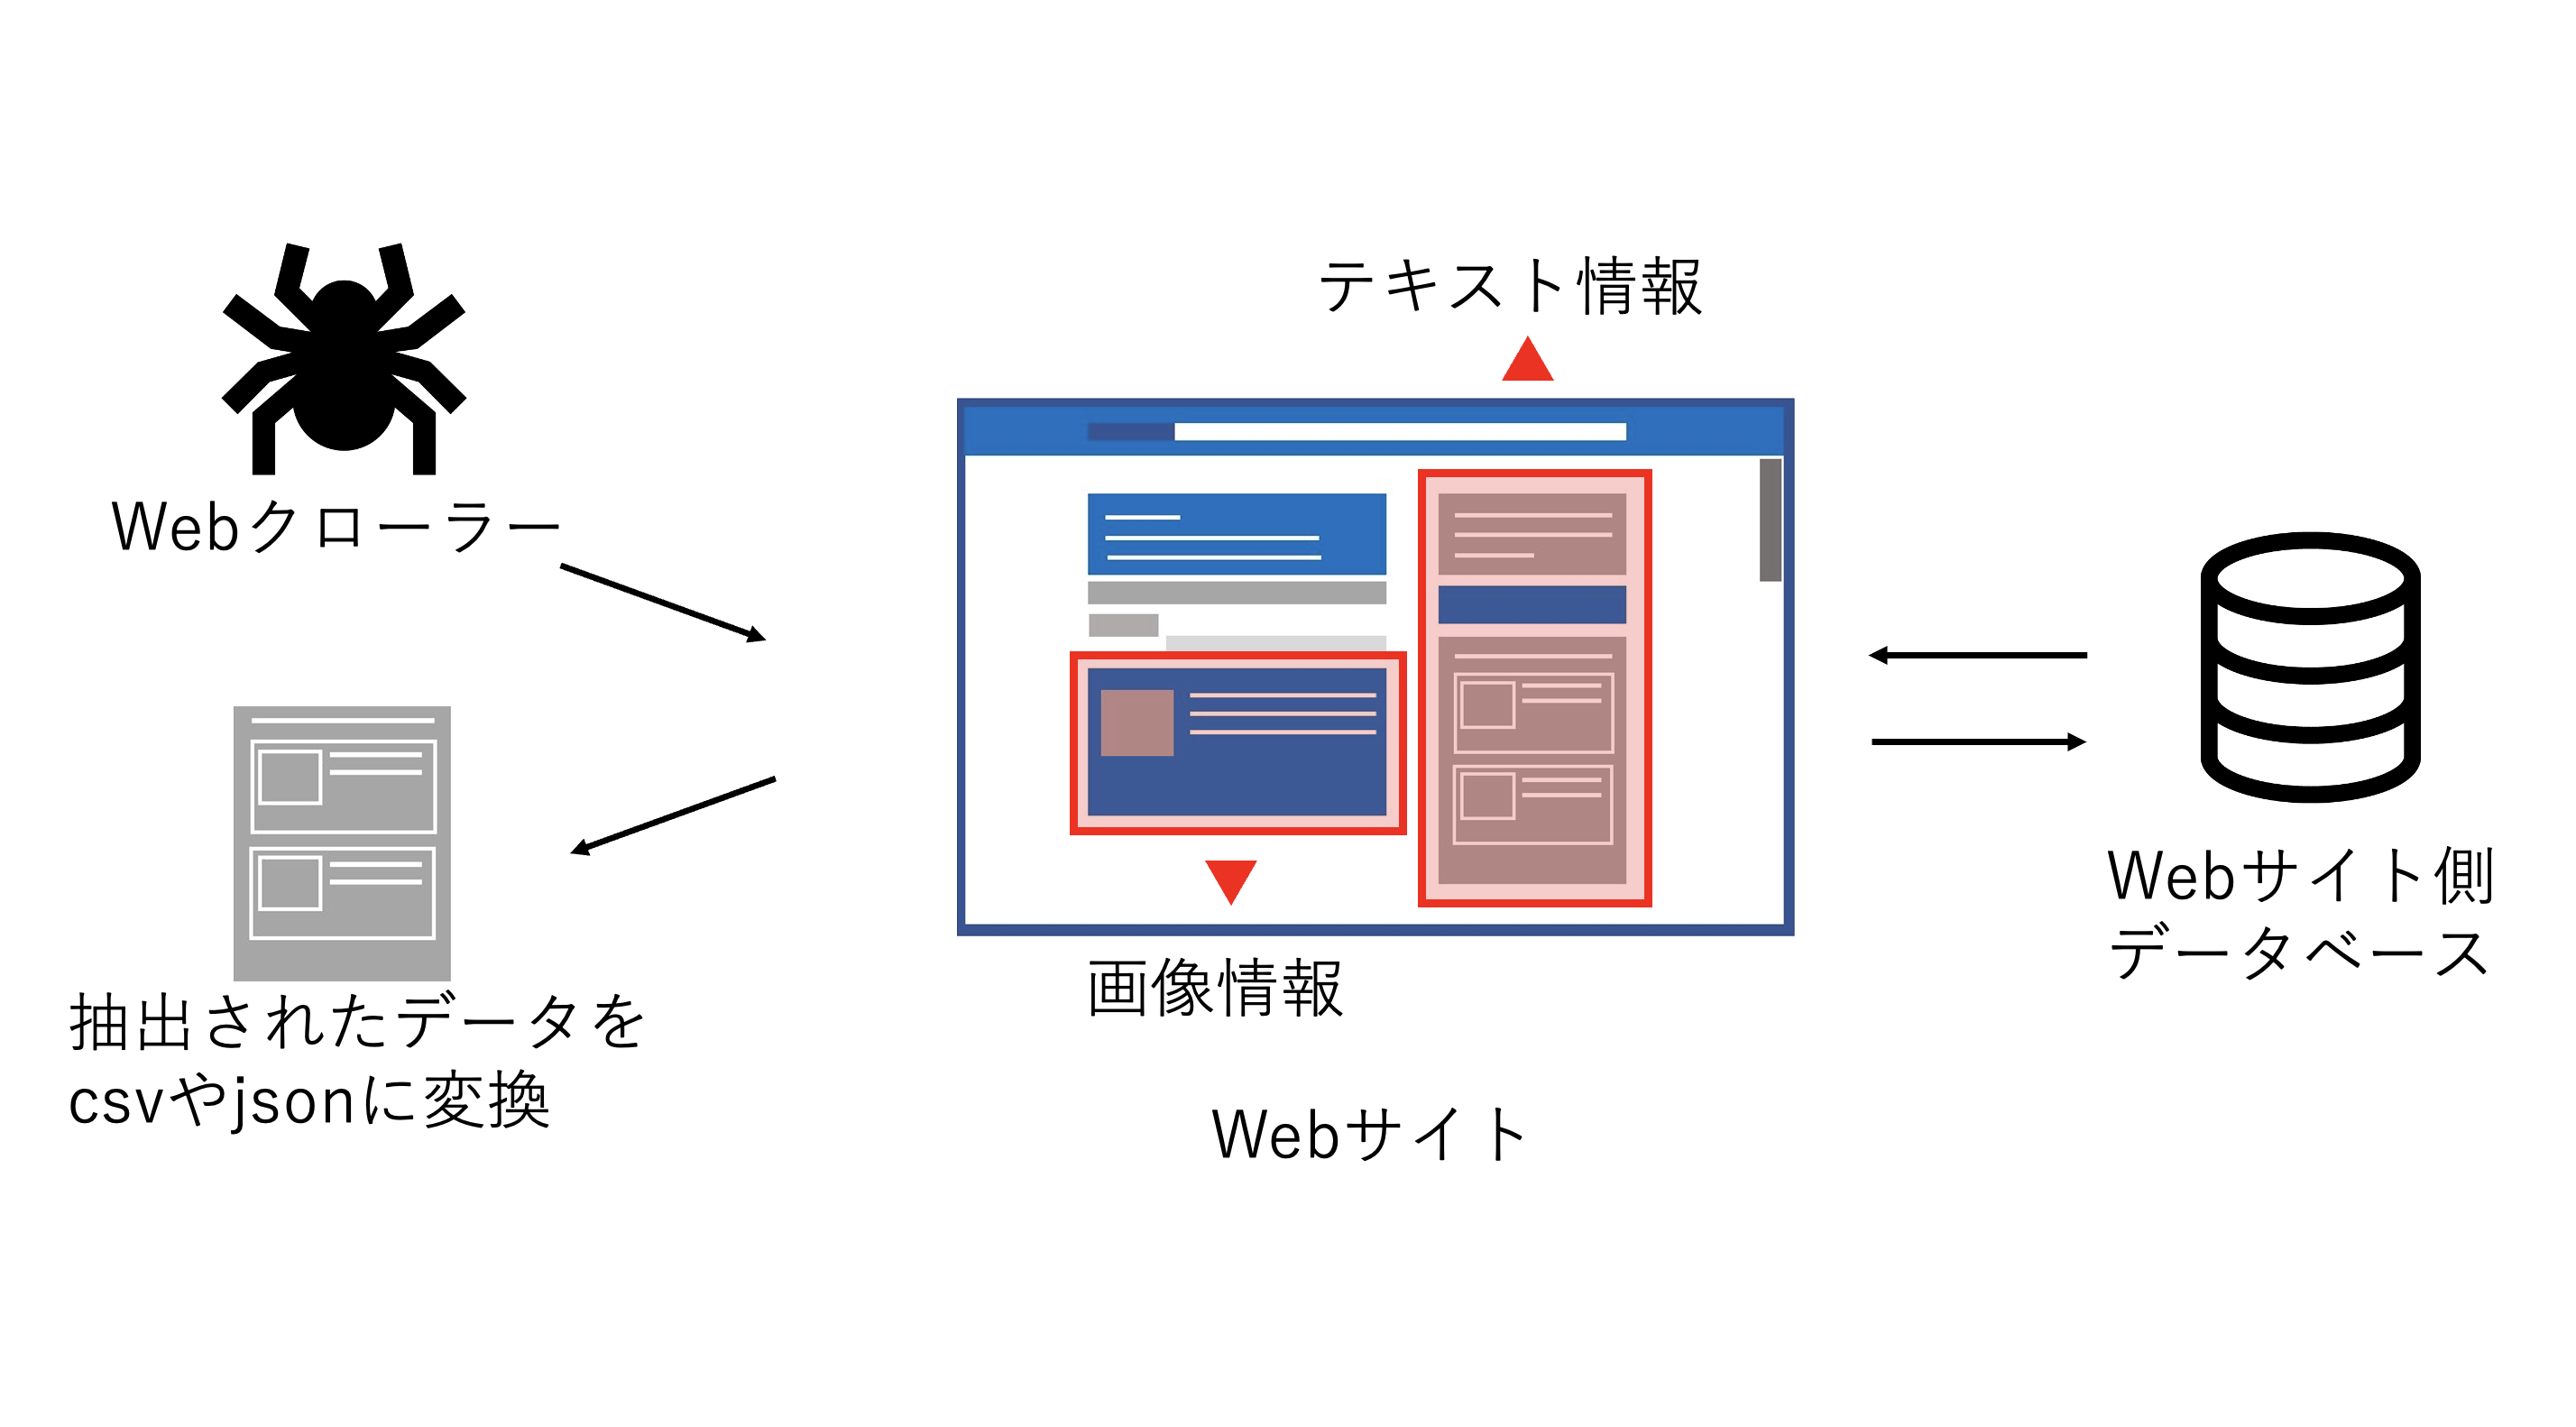
\includegraphics[width=0.9\linewidth]{./src/selenium.png}
	\caption{スクレイピングの解説}
  \label{fig:arch}
\end{figure}

\section{提案}



\section{実装}


\section{進捗と計画}


\section{まとめ}


\section{情報システムコースにおける本研究の位置づけ}


\begin{thebibliography}{99}
	\bibitem{rikkyo}
	立教大学, "立教大学シラバス検索システム", 立教大学. [Online]. Available from: \url{https://www.rep-rikkyo.com/class_rooms?day=c&hour=4}. Accessed: 2023-10-25.
	\bibitem{gakugei}
	東京学芸大学 (非公式), "東京学芸大学教室検索システム", 東京学芸大学. [Online]. Available from: \url{https://u-gakugei-uoa.pages.dev/akitan/}. Accessed: 2023-10-25.
	\bibitem{selenium}
	SeleniumHQ, "Selenium Documentation", Selenium, 2023. [Online]. Available from: \url{https://www.selenium.dev/documentation/en/}. Accessed: 2023-10-25.
\end{thebibliography}
\end{document}
%
%
% EOF 
